\documentclass{article}
\usepackage{amsmath}
\usepackage{physics}
\usepackage{graphicx}
\usepackage{tikz}
\usepackage{mdframed}  % Add this package for framed environments
\usepackage{float}     % For better figure placement control
\usepackage{booktabs}  % For professional-looking tables

% Define the answer environment
\newenvironment{answer}
    {\begin{mdframed}[linewidth=0.5pt,backgroundcolor=gray!5]
    \vspace{0.5em}}
    {\vspace{0.5em}\end{mdframed}}

% Define solution figure settings
\makeatletter
\newenvironment{solutionfigure}
    {\begin{figure}[H]
    \centering
    \setlength{\abovecaptionskip}{6pt}
    \setlength{\belowcaptionskip}{6pt}}
    {\end{figure}}
\makeatother

% Define solution table settings
\makeatletter
\newenvironment{solutiontable}
    {\begin{table}[H]
    \centering
    \setlength{\abovecaptionskip}{6pt}
    \setlength{\belowcaptionskip}{6pt}}
    {\end{table}}
\makeatother

\title{Exercise Set 1: Understanding Trajectory Probabilities}
\author{Supplementary Exercises for Maximum Caliber}
\date{}

\begin{document}
\maketitle

\section*{Exercise 1: Introduction to Path Probabilities}

Consider a particle that can move on a 1D discrete lattice with sites labeled by integers. At each time step, the particle can jump one step to the left or right.


\begin{enumerate}
    \item[(a)] Draw all possible 3-step trajectories starting from position x=0. For each trajectory, label the sequence of positions visited.

    \begin{answer}
    \begin{solutionfigure}
        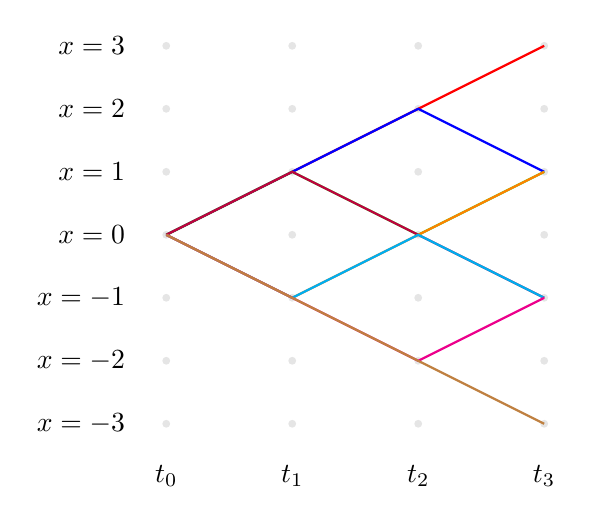
\begin{tikzpicture}[scale=0.8]
            % Grid
            \foreach \x in {-3,...,3}
                \foreach \t in {0,...,3}
                    \node[circle,fill=gray!20,inner sep=1pt] at (\t*2,\x) {};
            
            % Time labels
            \foreach \t/\label in {0/t_0,1/t_1,2/t_2,3/t_3}
                \node[below] at (\t*2,-3.5) {$\label$};
            
            % Position labels
            \foreach \y/\label in {-3/-3,-2/-2,-1/-1,0/0,1/1,2/2,3/3}
                \node[left] at (-0.5,\y) {$x=\label$};
            
            % Paths (using different colors for clarity)
            \draw[red,thick] (0,0) -- (2,1) -- (4,2) -- (6,3);
            \draw[blue,thick] (0,0) -- (2,1) -- (4,2) -- (6,1);
            \draw[green,thick] (0,0) -- (2,1) -- (4,0) -- (6,1);
            \draw[purple,thick] (0,0) -- (2,1) -- (4,0) -- (6,-1);
            \draw[orange,thick] (0,0) -- (2,-1) -- (4,0) -- (6,1);
            \draw[cyan,thick] (0,0) -- (2,-1) -- (4,0) -- (6,-1);
            \draw[magenta,thick] (0,0) -- (2,-1) -- (4,-2) -- (6,-1);
            \draw[brown,thick] (0,0) -- (2,-1) -- (4,-2) -- (6,-3);
        \end{tikzpicture}
        \caption{All possible 3-step trajectories starting from x=0.}
    \end{solutionfigure}
    \end{answer}
    \item[(b)] If the probability of jumping left is p and right is (1-p) at each step, write an expression for the probability of each trajectory you drew in part (a).
    \begin{answer}
        \begin{solutiontable}
            \begin{tabular}{lcc}
                & $\Gamma$ & $p(\Gamma)$ \\
                0 & LLL & ppp \\
                1 & LLR & pp(1-p) \\
                2 & LRL & p(1-p)p \\
                3 & LRR & p(1-p)(1-p) \\
                4 & RLL & (1-p)pp \\
                5 & RLR & (1-p)p(1-p) \\
                6 & RRL & (1-p)(1-p)p \\
                7 & RRR & (1-p)(1-p)(1-p)
            \end{tabular}
        \end{solutiontable}
    \end{answer}


    \item[(c)] Show that the sum of probabilities over all possible trajectories equals 1.
    \begin{answer}
        \begin{eqnarray}
            \sum_\Gamma p(\Gamma) & = p^3 + p^2(1-p) + (1-p)^2p + (1-p)^3 \nonumber \\
            & = (p + (1-p))^3 \nonumber \\
            & = 1 
        \end{eqnarray}
    \end{answer}
    \item[(d)] For a trajectory $\Gamma$ of $n$ steps, write a general expression for its probability $p_\Gamma$ in terms of the number of left steps $n_L$ and right steps $n_R$.
    \begin{answer}
        $$
        p(\Gamma) = \prod_{i=1}^n p^{s_i}(1-p)^{1-s_i}
        $$
        where $s_i$ is 1 if the $i$th move is left and 0 if it is right.
    \end{answer}
\end{enumerate}



\section*{Exercise 2: From Discrete to Continuous Paths}

\begin{enumerate}
    \item[(a)] Consider the limit where the time step $\Delta t \to 0$ and lattice spacing $\Delta x \to 0$ such that $(\Delta x)^2/\Delta t$ remains constant. Show that the discrete random walk approaches a continuous diffusion process.
    \begin{answer}
        In this limit we have a bionomial distribution where at time $t_j$ the location $x_j$ is given by
        \begin{eqnarray}
        x_j & = \sum_{i=1}^j \Delta x s_i - \sum_{i=1}^j \Delta x (1-s_i) \nonumber \\
        & = \Delta x\left(2 \sum_{i=1}^j s_i - j\right).
        \end{eqnarray}
        Because it's a sum over scaled bionomial variables, then we can apply the central limit theorem to find the mean and covariance of $x$.
        
        Expectation of $x_j$ is given by 
        $$
        \langle x_j\rangle = \Delta x j (2 p - 1).
        $$ 
        Taking $j=\frac{t}{\Delta t}$ we have 
        $$
        \langle x(t)\rangle = \frac{\Delta x}{\Delta t}(1- 2p)t
        $$ 
        which will be infinite unless $p=1/2$ so we have $\langle x(t)\rangle = 0$.
        
        Product of $x_j x_{j^\prime}$ is given by 
        $$
        x_j x_{j^\prime} = \Delta x^2 \left(4\sum_{i=1}^j s_i \sum_{{i^\prime}=1}^{j^\prime} s_{i^\prime} -j^\prime\sum_{i=1}^j s_i -j\sum_{{i^\prime}=1}^{j^\prime} s_{i^\prime} +jj^\prime\right).
        $$. Taking $j^\prime = j+\Delta j$ we have $\langle x_j x_{j^\prime}\rangle = \Delta x^2 p j (j+\Delta j) - \Delta x^2 (1-p) j (j+\Delta j)$.
    \end{answer}
    \item[(b)] For a continuous trajectory $x(t)$ over time interval $[0,T]$, explain why we write the probability functional as:
    \[ 
    P[x(t)] = \mathcal{N} \exp\left(-\frac{1}{4D}\int_0^T \left(\frac{\text{d}x}{\text{d}t}\right)^2 \text{d}t\right) 
    \]
    where $D$ is the diffusion coefficient and $\mathcal{N}$ is a normalization factor.
    \begin{answer}
    \end{answer}
    \item[(c)] How does this continuous probability functional relate to the discrete probability from Exercise 1(d)?
    \begin{answer}
        The discrete probability is given by $p(\Gamma) = \prod_{i=1}^n p^{s_i}(1-p)^{1-s_i}$.
    \end{answer}
\end{enumerate}

\section*{Exercise 3: Physical Observables and Path Ensembles}

Consider a general observable $A[x(t)]$ that depends on the entire trajectory.

\begin{enumerate}
    \item[(a)] Write an expression for the ensemble average $\langle A \rangle$ in terms of the path probability $P[x(t)]$.
    
    \item[(b)] For the specific case where $A[x(t)]$ is the average velocity over the trajectory:
    \[ 
    A[x(t)] = \frac{1}{T}\int_0^T \frac{dx}{dt} dt 
    \]
    show that $\langle A \rangle = 0$ for the probability functional given in Exercise 2(b).
    
    \item[(c)] If we now add a constant force $F$, the probability functional becomes:
    \[ 
    P[x(t)] = \mathcal{N} \exp\left(-\frac{1}{4D}\int_0^T \left[\left(\frac{\text{d}x}{\text{d}t}\right)^2 - \frac{2F}{m}\frac{\text{d}x}{\text{d} t}\right] \text{d}t\right) 
    \]
    Calculate $\langle A \rangle$ in this case.

    \item[(d)] Consider the integral in the exponent of the probability functional from part (c).
    \begin{enumerate}
        \item[(i)] Show that the most probable path maximizes this probability by minimizing this integral.
        \item[(ii)] Multiply the integrand by $-4D$ and compare it with the classical Lagrangian $L = \frac{1}{2}m\dot{x}^2 + Fx$. What do you notice?
        \item[(iii)] Using this comparison, show that the most probable path satisfies Newton's equation of motion $m\ddot{x} = F$. What does this tell us about the relationship between maximum probability and least action?
    \end{enumerate}
\end{enumerate}

\section*{Exercise 4: Connection to Maximum Caliber}

\begin{enumerate}
    \item[(a)] Compare the probability functional in Exercise 2(b) with the MaxCal form:
    \[ p_\Gamma = \frac{q_\Gamma}{Z}\exp\left(\sum_t \lambda(t)j_\Gamma(t)\right) \]
    Identify the corresponding terms and explain their physical meaning.
    
    \item[(b)] Explain why the reference distribution $q_\Gamma$ in MaxCal corresponds to the equilibrium distribution. What role does it play in determining the most probable trajectories?
    
    \item[(c)] Show that when $\lambda(t)=0$, the MaxCal distribution reduces to the equilibrium distribution and there are no net currents.
\end{enumerate}

\section*{Exercise 5: Quantum-Classical Correspondence}

The Feynman path integral in quantum mechanics gives the probability amplitude for a particle to go from position $x_a$ at time $t_a$ to position $x_b$ at time $t_b$:
\[
K(x_b,t_b;x_a,t_a) = \int \mathcal{D}x(t) \exp\left(\frac{i}{\hbar}\int_{t_a}^{t_b} \left[\frac{m}{2}\left(\frac{dx}{dt}\right)^2 - V(x)\right]dt\right)
\]
where $\mathcal{D}x(t)$ represents integration over all possible paths.

\begin{enumerate}
    \item[(a)] Show that under a Wick rotation $t \to -i\tau$, the Feynman path integral for quantum mechanics transforms into the form given in Exercise 2(b) with $D = \frac{\hbar}{2m}$.
    
    \item[(b)] Calculate the variance in position $\langle x^2(t) \rangle$ for both the classical diffusion process and the quantum case. What does this tell you about the relationship between diffusion and quantum uncertainty?
    
    \item[(c)] Using this correspondence, explain why the classical probability distribution $P[x(t)]$ can be interpreted as a Euclidean quantum amplitude. What are the limitations of this interpretation?
    
    \item[(d)] Show that in the limit $\hbar \to 0$, the most probable path from the quantum path integral reduces to the classical path that minimizes the action. How does this relate to the principle of least action?
\end{enumerate}

\section*{Exercise 6: MaxCal and Schrödinger's Bridge}

\begin{enumerate}
    \item[(a)] Consider the MaxCal principle with constraints on both initial $\rho_0(x)$ and final $\rho_1(x)$ distributions:
    \[ 
    p[\Gamma] = \frac{1}{Z}\exp\left(-\int_0^1 L(x,\dot{x})dt + \lambda_0(x(0)) + \lambda_1(x(1))\right) 
    \]
    Show that this leads to a modified ``action'':
    \[ 
    S_{eff}[\Gamma] = \int_0^1 L(x,\dot{x})dt - \ln\rho_0(x(0)) - \ln\rho_1(x(1)) 
    \]

    \item[(b)] Demonstrate that minimizing the relative entropy:
    \[ 
    D(P\|Q) = \int \mathcal{D}x P[x(t)]\ln\frac{P[x(t)]}{Q[x(t)]} 
    \]
    subject to the endpoint constraints gives the same form as Schrödinger's bridge problem.

    \item[(c)] Show that the resulting optimal dynamics can be written as:
    \[ 
    \frac{\text{d}x}{\text{d}t} = b(x,t) + D\nabla\ln\psi(x,t) 
    \]
    where $\psi(x,t)$ satisfies a forward-backward system of equations.
\end{enumerate}

\end{document} 